\documentclass[12pt]{article}
\usepackage{graphicx} % Required for inserting images
\usepackage[margin=0.5in]{geometry}
\usepackage{amsmath, amssymb}
\usepackage{mathrsfs}


\usepackage{soul}


% Dr. David Brown Commands
\newcommand{\ds}{\displaystyle}
\newcommand{\R}{\mathbb{R}}
\newcommand{\N}{\mathbb{N}}
\newcommand{\Q}{\mathbb{Q}}
\newcommand{\C}{\mathbb{C}}


% Commands to get script r
\usepackage{calligra}
\DeclareMathAlphabet{\mathcalligra}{T1}{calligra}{m}{n}
\DeclareFontShape{T1}{calligra}{m}{n}{<->s*[2.2]callig15}{}
\newcommand{\scripty}[1]{\ensuremath{\mathcalligra{#1}}}

% Unit commands
\newcommand{\degree}{\text{°}}
\newcommand{\unitSpeed}{\frac{\text{m}}{\text{s}}}
\newcommand{\unitAcceleration}{\frac{\text{m}}{\text{s}^2}}

% Constant commands
\newcommand{\avogadro}{6.022\times10^{23}}

\newcommand{\boltzmannConstK}{1.381\times10^{-23}\frac{\text{J}}{\text{K}}}
\newcommand{\boltzmannConstInEV}{8.617\times10^{-5}\frac{\text{eV}}{\text{K}}}
\newcommand{\planckConst}{6.626\times10^{-34}\text{J}\cdot\text{s}}

\newcommand{\atmP}{1.01325\times10^5\,\text{Pa}}

% Commands to easily write partial derivatives
\newcommand{\partDeriv}[2]{\frac{\partial #1}{\partial #2}}
\newcommand{\doublePartDeriv}[2]{\frac{\partial^2 #1}{\partial^2 #2}}


\title{Problem 6.16}
\author{Gabriel Decker}


\begin{document}



\maketitle
\begin{flushleft}

Starting off, we know the following definitions of $\overline{E}$, $Z$, and total energy $U$.

\begin{equation}
    \overline{E}=-\partDeriv{}{\beta}\ln(Z)
\end{equation}
\begin{equation}
    Z=\sum_se^{-\beta E(s)}
\end{equation}
\begin{equation}
    U=N\overline{E}
\end{equation}
where $\beta=1/kT$.\\~\\


\textbf{Part a}\\
First, we must show by long division the following.
$$\frac{1}{1-x}=1+x+x^2+x^3+\dots$$

Here is my work (it's hard to do long division in LaTeX)\\
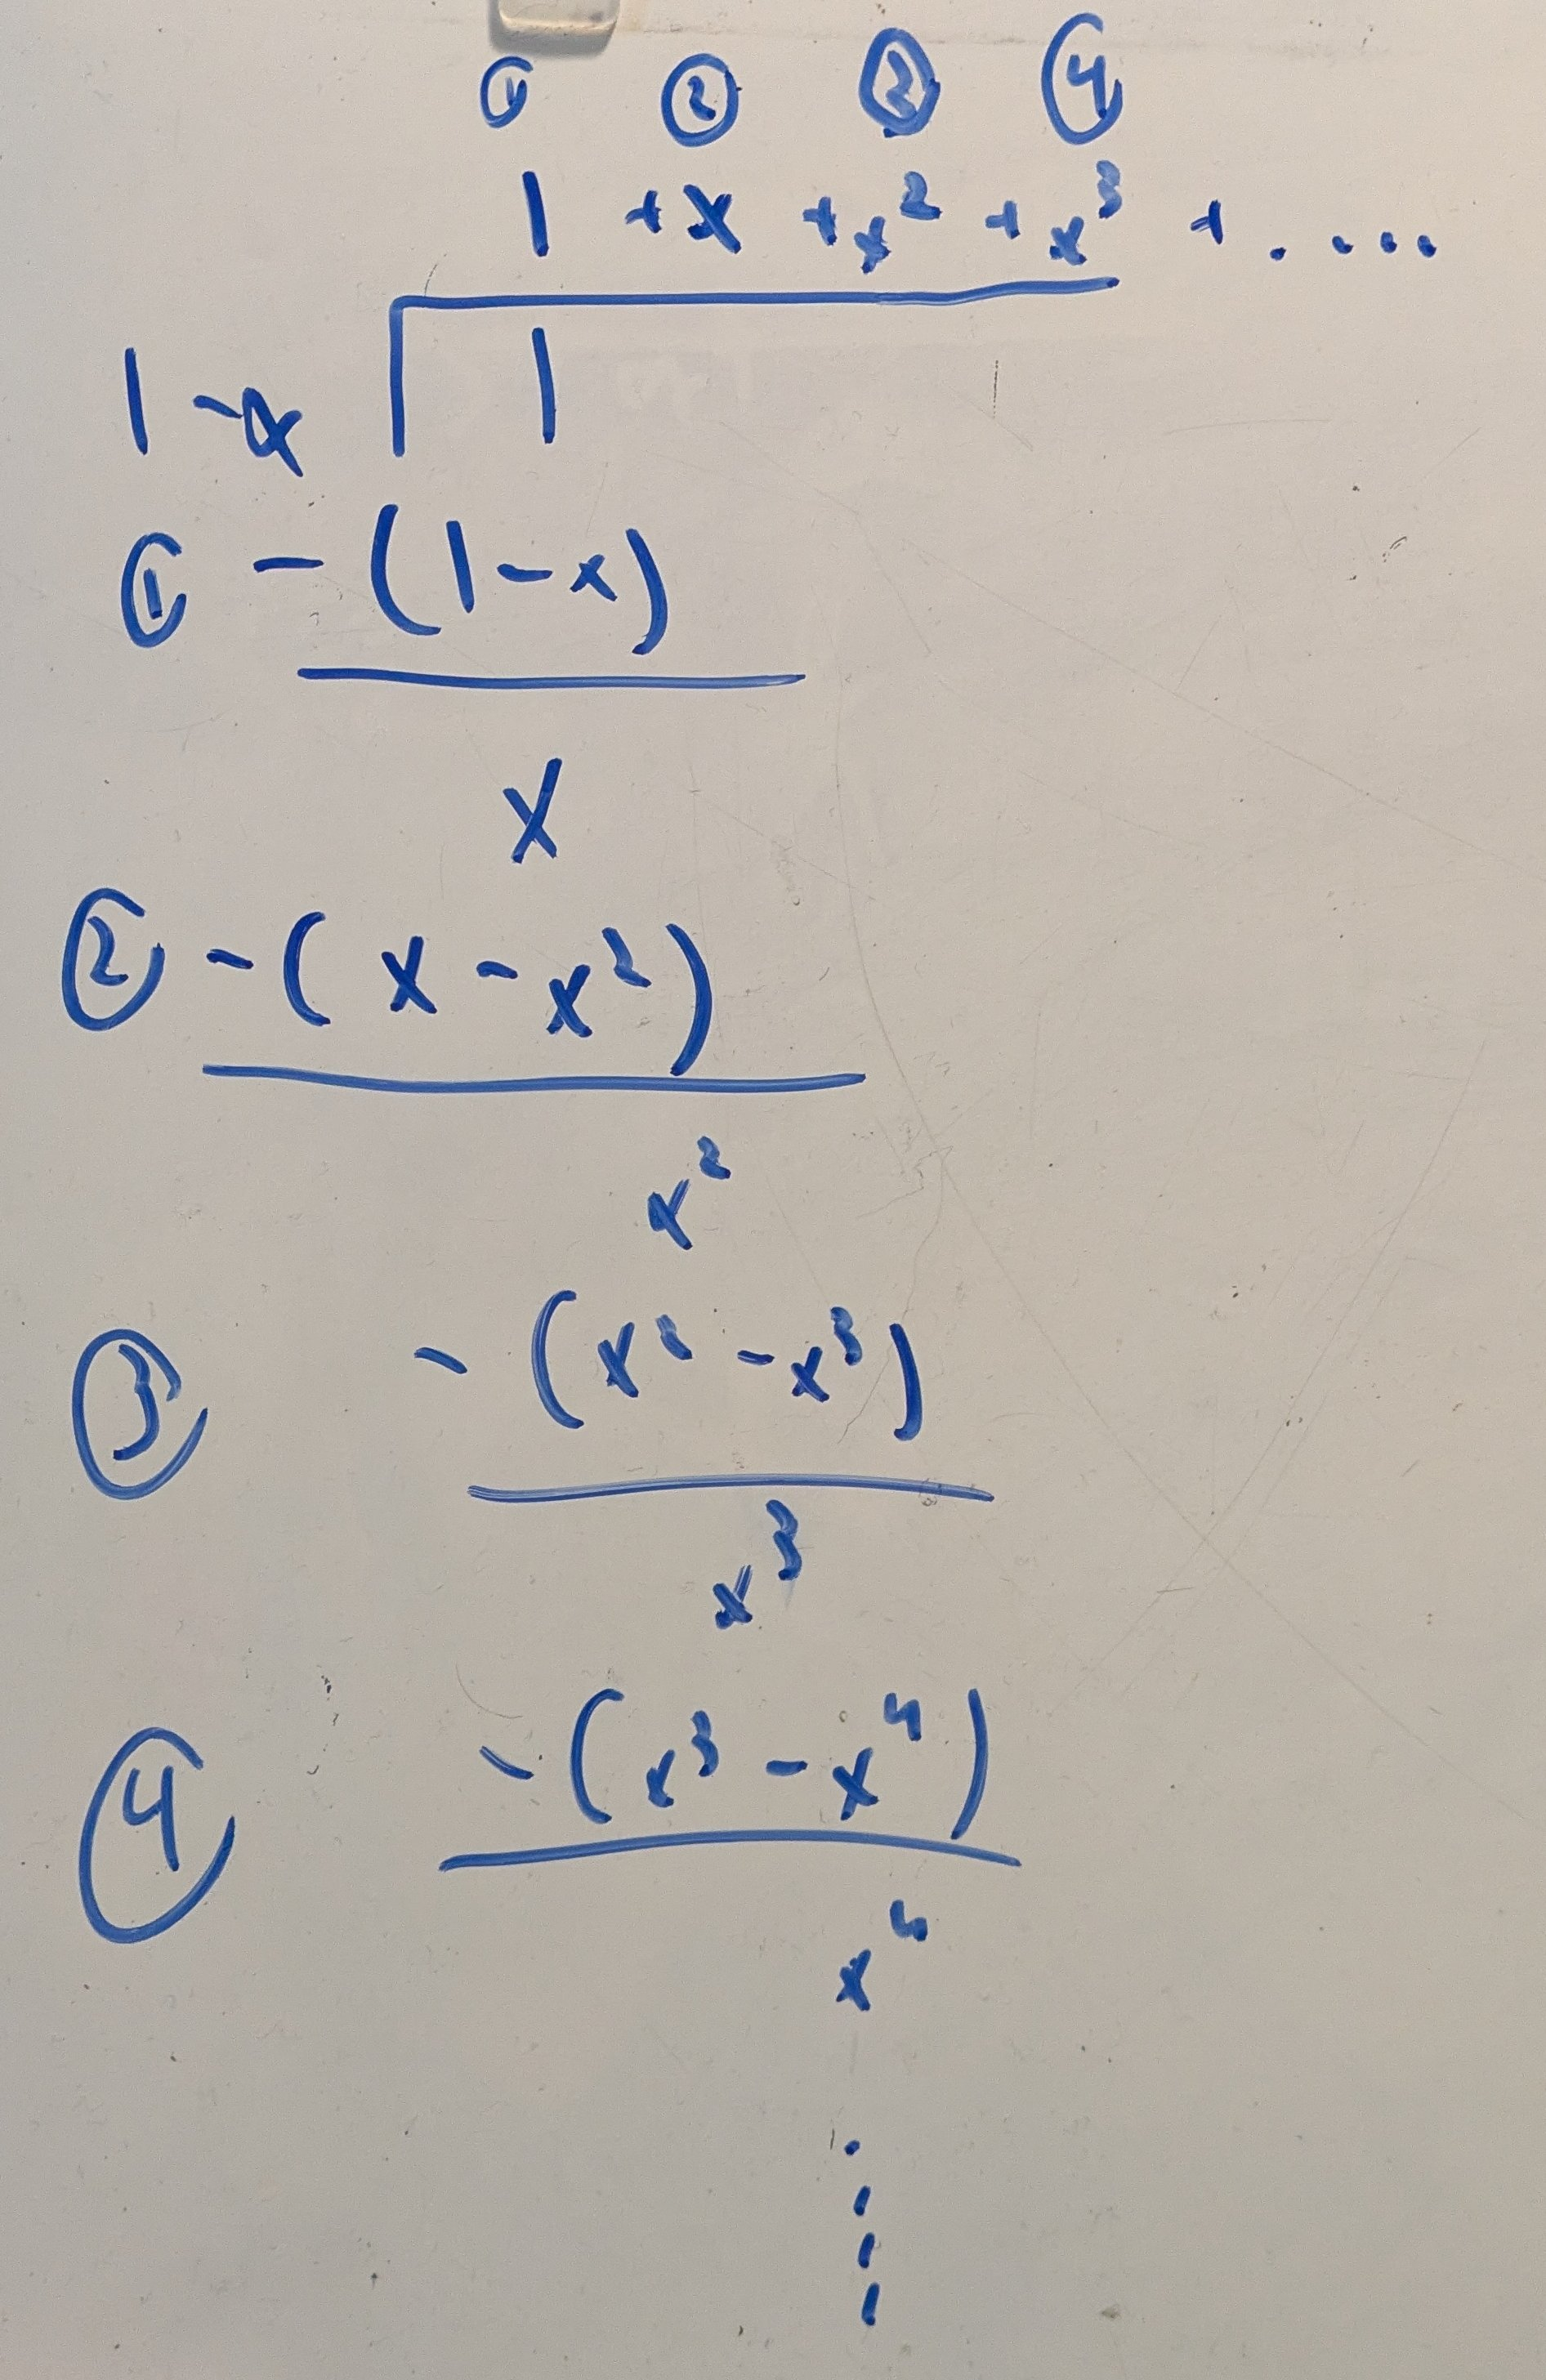
\includegraphics[width=0.4\linewidth]{long_division.jpg}\\
With this, it's clear that to continue getting rid of the remaining term, you must continually add a term with higher and higher power.
This is an example of a geometric series, and as such, has a finite sum when $|x|<1$.\\~\\

\textbf{Part b}\\
Now, we must evaluate the partition function $Z$ for our system of $N$ harmonic oscillators at temperature $T$. The possible energies are nonnegative integer multiples of $hf$.
For this, we use the equation of $Z$. We can plug in the various energies we have.
$$Z=\sum_se^{-\beta E(s)}$$
$$\implies Z=\sum_{n=0}^\infty e^{-n\beta hf}$$
Expanding this out a bit, we can see a familiar pattern.
$$\implies Z\approx e^{-0\beta hf}+e^{-1\beta hf}+e^{-2\beta hf}+e^{-3\beta hf}+\dots$$
$$\implies Z\approx 1+(e^{-\beta hf})^1+(e^{-\beta hf})^2+(e^{-\beta hf})^3+\dots$$
Since $e$ to the power of any negative exponent has the range $(0,1)$, this implies that this infinite sum converges to the following.
$$\implies Z=\frac{1}{1-e^{-\beta hf}}$$\\~\\


\textbf{Part c}\\
Now that we have an expression for the partition function $Z$, we can easily find $\overline{E}$.
$$\overline{E}=-\partDeriv{}{\beta}\ln(Z)$$
$$\implies\overline{E}=-\frac{1}{Z}\partDeriv{Z}{\beta}$$
$$\implies\overline{E}=-(1-e^{-\beta hf})\partDeriv{}{\beta}(\frac{1}{1-e^{-\beta hf}})$$
$$\implies\overline{E}=-(1-e^{-\beta hf})\partDeriv{}{\beta}((1-e^{-\beta hf})^{-1})$$
$$\implies\overline{E}=(1-e^{-\beta hf})(1-e^{-\beta hf})^{-2}\partDeriv{}{\beta}(1-e^{-\beta hf})$$
$$\implies\overline{E}=(1-e^{-\beta hf})(1-e^{-\beta hf})^{-2}(hfe^{-\beta hf})$$
$$\implies\overline{E}=\frac{hfe^{-\beta hf}}{1-e^{-\beta hf}}$$\\~\\


\textbf{Part d}\\
The total energy of a system at temperature $T$ with $N$ oscillators is simply
$$U=N\overline{E}$$
$$\implies U=N\frac{hfe^{-\beta hf}}{1-e^{-\beta hf}}$$
$$\implies U=Nhf\frac{e^{-\beta hf}}{1-e^{-\beta hf}}\cdot\frac{1/e^{-\beta hf}}{1/e^{-\beta hf}}=\frac{Nhf}{e^{\beta hf}-1}$$\\~\\


\textbf{Part e}\\
For this problem, we must find the heat capacity, given some temperature.
This can be done by using the following formula.
\begin{equation}
    C_V=\partDeriv{U}{T}
\end{equation}
Recall that $\beta=1/kT$.
Plugging in our expression for $U$ leads to the following.
$$C_V=\partDeriv{U}{T}$$
$$\implies C_V=\partDeriv{}{T}(\frac{Nhf}{e^{\beta hf}-1})$$
$$\implies C_V=Nhf\partDeriv{}{T}((e^{hf/kT}-1)^{-1})$$
$$\implies C_V=-Nhf(e^{hf/kT}-1)^{-2}\partDeriv{}{T}(e^{hf/kT}-1)$$
$$\implies C_V=-Nhf(e^{hf/kT}-1)^{-2}e^{hf/kT}\partDeriv{}{T}(hf/kT)$$
$$\implies C_V=Nhf(e^{hf/kT}-1)^{-2}e^{hf/kT}\frac{hf}{kT^2}$$
$$\implies C_V=\frac{N(hf)^2e^{hf/kT}}{kT^2(e^{hf/kT}-1)^2}$$\\~\\

Now that we have this equation for heat capacity $C_V$, we can examine how limits of temperature affect it. We'll check $T\rightarrow0$ and $T\rightarrow\infty$. Before doing this, we'll make the following change of variables to simplify the math.\\~\\

$$x=\frac{hf}{kT}$$
$$\implies T=\frac{hf}{kx}$$
$$\implies T^2=\frac{(hf)^2}{(kx)^2}$$
Plugging this into our equation for $C_V$, we get the following.
$$\implies C_V=\frac{Nkx^2e^x}{(e^x-1)^2}$$\\~\\

$T\rightarrow0$:\\
Because of the definition of $x$, $T\rightarrow0\implies x\rightarrow\infty$.
$$C_V(x\rightarrow\infty)=\lim_{x\rightarrow\infty}\left(\frac{Nkx^2e^x}{(e^x-1)^2}\right)$$
The $-1$ is irrelevant compared to the functional infinity, so
$$\implies C_V(x\rightarrow\infty)=\lim_{x\rightarrow\infty}\left(Nk\frac{x^2e^x}{(e^x)^2}\right)$$
$$\implies C_V(x\rightarrow\infty)=\lim_{x\rightarrow\infty}\left(Nk\frac{x^2}{e^x}\right)=Nk\frac{\infty}{\infty}$$
This is an indeterminate form, but applying L'Hopital's rule twice, we get the following.
$$\implies C_V(x\rightarrow\infty)=\lim_{x\rightarrow\infty}\left(Nk\frac{2x}{e^x}\right)=Nk\frac{\infty}{\infty}$$
$$\implies C_V(x\rightarrow\infty)=\lim_{x\rightarrow\infty}\left(\frac{2Nk}{e^x}\right)=0$$

$T\rightarrow\infty$:\\
Because of the definition of $x$, $T\rightarrow\infty\implies x\rightarrow0$.
$$C_V(x\rightarrow0)=\lim_{x\rightarrow0}\left(\frac{Nkx^2e^x}{(e^x-1)^2}\right)$$
This can be simplified by using the Taylor expansion of $e^x$, which for small $x$ can be approximated as $e^x\approx1+x$.
$$\implies C_V(x\rightarrow0)\approx\lim_{x\rightarrow0}\left(\frac{Nkx^2e^x}{(1-x-1)^2}\right)$$
$$\implies C_V(x\rightarrow0)=\lim_{x\rightarrow0}\left(\frac{Nkx^2e^x}{x^2}\right)$$
$$\implies C_V(x\rightarrow0)=\lim_{x\rightarrow0}\left(Nke^x\right)$$
$$\implies C_V(x\rightarrow0)=Nk$$


\end{flushleft}

\end{document}
